\subsection{Differential gears} \label{sec:Differentialgears}

The differential gear box is located as the first component in the drivetrain, after the connection to the motor (Part 2 on \figref{vehicleDescriptionDriveTrain} in \secref{sec:Vehicledescription}).
When the servo is braking on one of the sides of the drivetrain, the differential gears transfer the rotational energy from the side, where the brake is triggered, to the other side. This keep the lose of energy for braking one side smaller, because the energy is instead transferred to the other belt. The extra speed on the other belt, that is not braking, will make the vehicle turn faster, compared to if the rotational energy was not transferred.

A differential gear system can be seen on \figref{diffGearLight}

\begin{figure}[H]
	\centering
	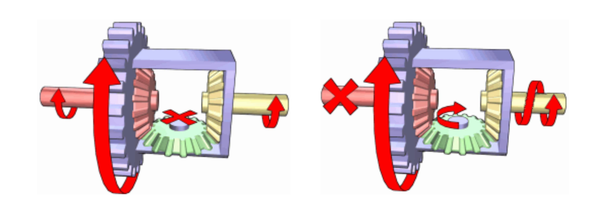
\includegraphics[scale=0.7]{figures/diffGearLight}
	\caption{Illustration to a differential gear system. At the left, the load on each side is equal, so the spider gear does not rotated. At the right, the load on the left side is not moving, because of a big load, so the spider gear rotates and transfer more rotational energy to the right side. \cite{MechanicalEngineering}}
	\label{diffGearLight}
\end{figure}

The differential gear system contains a ring gear (blue), a spider gear (green), two side gears to the rest of the system (yellow and red) and a pinion gear, that transfer the power from the motor to the system (not shown on picture, but is connected to the ring gear).\\

When the motor is running, the pinion gear transfer a rotation energy to the ring gear. The ring gear and the spider gear, that is fixed on to the ring gear, begins to rotate around the side gear from this energy. If the resistance on both side gears is the same, there is none difference in the power there is needed to rotate the gear. Therefore will the spider gear not rotate around it own axis and only be spin around be the ring gear and apply the same rotational energy to each side gear.\\

When the resistance on both sides is not equal to each other, i.g. if one of the side is being brake on, the spider gear will rotate around is own axis. This is because there is a bigger resistance one side than the other, so the side not braking will be easier to rotate. So the ring gear and spider gear is rotating at the same speed around the two side gears, but the spider gear will apply less rotational energy to the braking side and more to the none braking side, because of it own rotation. In the case that the resistance on one side is infinite, the spider gear will be rotating at the same speed as the ring gear. The side gear on the none braking side will therefore rotate twice as fast, with the assumption that there is no loss in the system.\\

For the differential gear system on the vehicle, there is a different setup, shown on \figref{diffGearFull}
	%\caption{Illustration of the differential gear system on the vehicle \cite{MechanicalEngineering}}

\begin{minipage}{\linewidth}
      \centering
      \begin{minipage}{0.65\linewidth}
          \begin{figure}[H]
              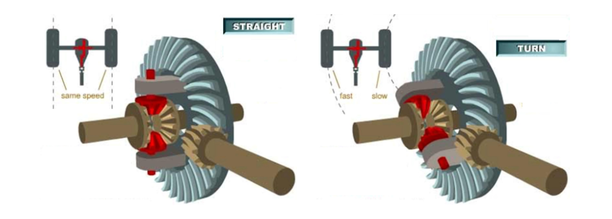
\includegraphics[width=0.95\textwidth]{figures/diffGearFull}
              \caption{Illustration of the differential gear system on the vehicle \cite{MechanicalEngineering}}
          \end{figure}
      \end{minipage}
      \hspace{0.05\linewidth}
      \begin{minipage}{0.25\linewidth}
      		\begin{enumerate}
      			\item Pinion gear
      			\item Ring gear
      			\item Spider gears
      			\item Side gears
      		\end{enumerate}
      \end{minipage}
  \end{minipage}




%\begin{table} [H]
%\begin{tabular}{p{3cm} p{3cm}}

%\begin{figure}
%	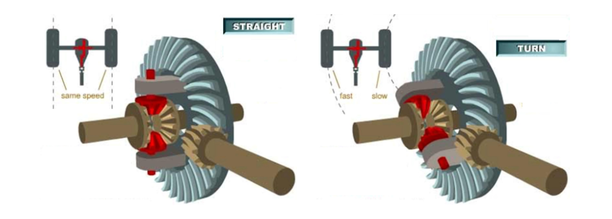
\includegraphics[scale=0.7]{figures/diffGearFull}
%	\label{diffGearFull}
%\end{figure}

%&

%\begin{enumerate}
 % \item Hallo
%\end{enumerate}

%\end{tabular}
%\end{table}




%\begin{figure} [h]
%	\centering
%	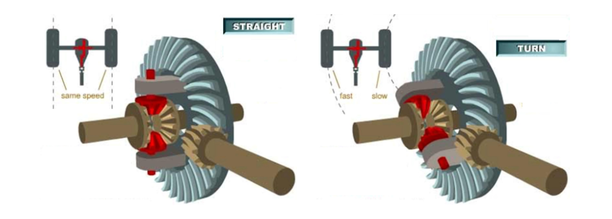
\includegraphics[scale=0.7]{figures/diffGearFull}
%	\caption{Illustration of the differential gear system on the vehicle \cite{MechanicalEngineering}}
%	\label{diffGearFull}
%\end{figure}

Instead of only having one spider gear (the green gear on \figref{diffGearLight}) there is two, shown in red on \figref{diffGearFull}. The system works in the same way as with one spider gear, with the pinion gear (1) transfer the power to the ring gear (2). The spider gears (3) rotates around with the ring gear and rotates the side gears (4) compare to the difference in their resistance.

Now that the vehicle has been presented and its limits analysed, the prototype contraints can be considered to aim the functionnalities needed in this project.

